\documentclass[12pt]{article}
\usepackage{tabularx}
\usepackage{amsmath} 
\usepackage{graphicx}
\usepackage[margin=1in]{geometry}
\usepackage{cite}
\usepackage[final]{hyperref}
\hypersetup{
	colorlinks=true,      
	linkcolor=blue,       
	citecolor=blue,       
	filecolor=magenta,    
	urlcolor=blue         
}
\usepackage{blindtext}
\usepackage{amssymb}
\usepackage{esint}
\usepackage{tikz}
\usepackage{pgfplots}
\usepackage{gensymb}
\usetikzlibrary{datavisualization}
\usetikzlibrary{datavisualization.formats.functions}
\newcommand{\Prho}{.8}%
\newcommand{\Ptheta}{55}%
\newcommand{\Pphi}{60}%
\usepackage{tikz-3dplot}
\newcommand{\uvec}[1]{\boldsymbol{\hat{\textbf{#1}}}}
%++++++++++++++++++++++++++++++++++++++++
\usepackage{empheq}

\newcommand*\widefbox[1]{\fbox{\hspace{2em}#1\hspace{2em}}}

\begin{document}

\usetikzlibrary{scopes}
\def\iangle{35} % Angle of the inclined plane

\def\down{-90}
\def\arcr{0.5cm} % Radius of the arc used to indicate angles

\title{ECE 3030 - HW 9}
\author{Joshua Tensuan - jvt24}
\date{November 18, 2022}
\maketitle


Code is also attached in separate file.
\begin{enumerate}
	\item [9.1]
	\begin{enumerate}
		\item [a.]
		Let $z=0$ be the position of the interface between the single dielectric layer and the silicon substrate, and $z=-\lambda/4$ be the position of the interface between the single dielectric layer and the vacuum environment.
		Then, we know that the normalized impedance at $z=0$ is given by,
		\[\eta_n(z=0)=\frac{\eta(z=0)}{\eta_2}=\frac{\eta_3}{\eta_2}=\frac{1+\Gamma_2}{1-\Gamma_2}\]
		where $\eta_i$ denotes the impedance of the $i$-th layer.
		Then,
		\[\eta_n(z=-l)=\frac{1+\Gamma_2e^{-2jk_2l}}{1-\Gamma_2e^{-2jk_2l}}\]
		If $l=\lambda_2/4$, $e^{-2jk_2l}=e^{-2j(2\pi/\lambda)(\lambda_2/4)}=e^{-j\pi}=-1$.
		Thus,
		\[\eta_n(z=-\lambda_2/4)=\frac{1-\Gamma_2}{1+\Gamma_2}=\frac{1}{\eta_n(z=0)}=\frac{\eta_2}{\eta_3}\]
		Then, using the fact that $\eta=\eta_2\eta_n$,
		\[\eta(z=-\lambda_2/4)=\frac{\eta_2^2}{\eta_3}\]
		In order to properly load match, we want,
		\[\Gamma_1 = 0 \to \frac{\eta(z=-\lambda_2/4)-\eta_1}{\eta(z=-\lambda_2/4)+\eta_1}=0\]
		\[\to \eta(z=-\lambda_2/4)=\eta_1 \to \frac{\eta_2^2}{\eta_3}=\eta_1\to \eta_2=\sqrt{\eta_1\eta_3}\]
		We know that wave impedance is given by,
		\[\eta=\sqrt{\frac{\mu_0}{\epsilon}}=\sqrt{\frac{\mu_0}{\epsilon_0}}\sqrt{\frac{\epsilon_0}{\epsilon}}=\frac{1}{n}\eta_0\]
		Substituting this into our impedance-matching equation,
		\[\frac{1}{n_2}\eta_0=\sqrt{\frac{1}{n_1}\frac{1}{n_3}\eta_0^2}\]
		\[\to \frac{1}{n_2}=\sqrt{\frac{1}{n_1n_3}}\to n_2=\sqrt{n_1n_3}\]
		Substituting in values for index of refraction,
		\[n_2=\sqrt{1\cdot 3.5} = 1.871\]
		To find the wavelength $\lambda_2$, we can use the fact that,
		\[k_2=n_2k_1\to \frac{2\pi}{\lambda_2}=n_2\frac{2\pi}{\lambda_1}\]
		\[\to \lambda_2=\frac{\lambda_1}{n_2}=\frac{0.52 \: \mu\mathrm{m}}{1.871}=0.278 \: \mu \mathrm{m}\]
		We said the dielectric layer should be $\lambda_2/4$ thick so,
		\[L_2 = \frac{0.278 \: \mu\mathrm{m}}{4}=0.0695\: \mu \mathrm{m}=6.95 \cdot 10^{-8}\:\mathrm{m}\]
		Thus, we have,
		\[\boxed{\begin{cases}
			n_2=1.871 \\ 
			L_2 = 6.95 \cdot 10^{-8}\:\mathrm{m}
		\end{cases}}\]

		\item [(b)]
		Defining $\Gamma_2$ as,
		\[\Gamma_2= \frac{\eta_3-\eta_2}{\eta_3+\eta_2}\]
		Substituting in appropriate values for $\eta$ with $\eta=\eta_0/n$ via Mathematica, we find that,
		\[\Gamma_2 = -0.303\]
		We know that via the impedance transformation equation,
		\[\eta(z=-L_2)=\eta_2\frac{1+\Gamma_2e^{-2j(2\pi/\lambda)L_2}}{1-\Gamma_2e^{-2j(2\pi/\lambda)L_2}}\]
		We know that the $\lambda$ in the small layer is given by, $\lambda_1/n_2$.
		Thus, we can rewrite $\eta(z=-L_2)$ as,
		\[\eta(z=-L_2)=\eta_2\frac{1+\Gamma_2e^{jC/\lambda_1}}{1-\Gamma_2e^{jC/\lambda_1}}\]
		where,
		\[C=-2\cdot \frac{2\pi\lambda_1}{\lambda}L_2=-\frac{4\pi\lambda_1}{\lambda_1}n_2L_2=-4\pi n_2L_2\]
		Then, $\Gamma_1=\frac{\eta(z=-L_2)-\eta_1}{\eta(z=-L_2)+\eta_1}$.
		We can generate a plot for $|\Gamma_1|^2$ over the range of $\lambda_1:[0.3,0.9]\:\mu\mathrm{m}$ with the below Python snippet,

		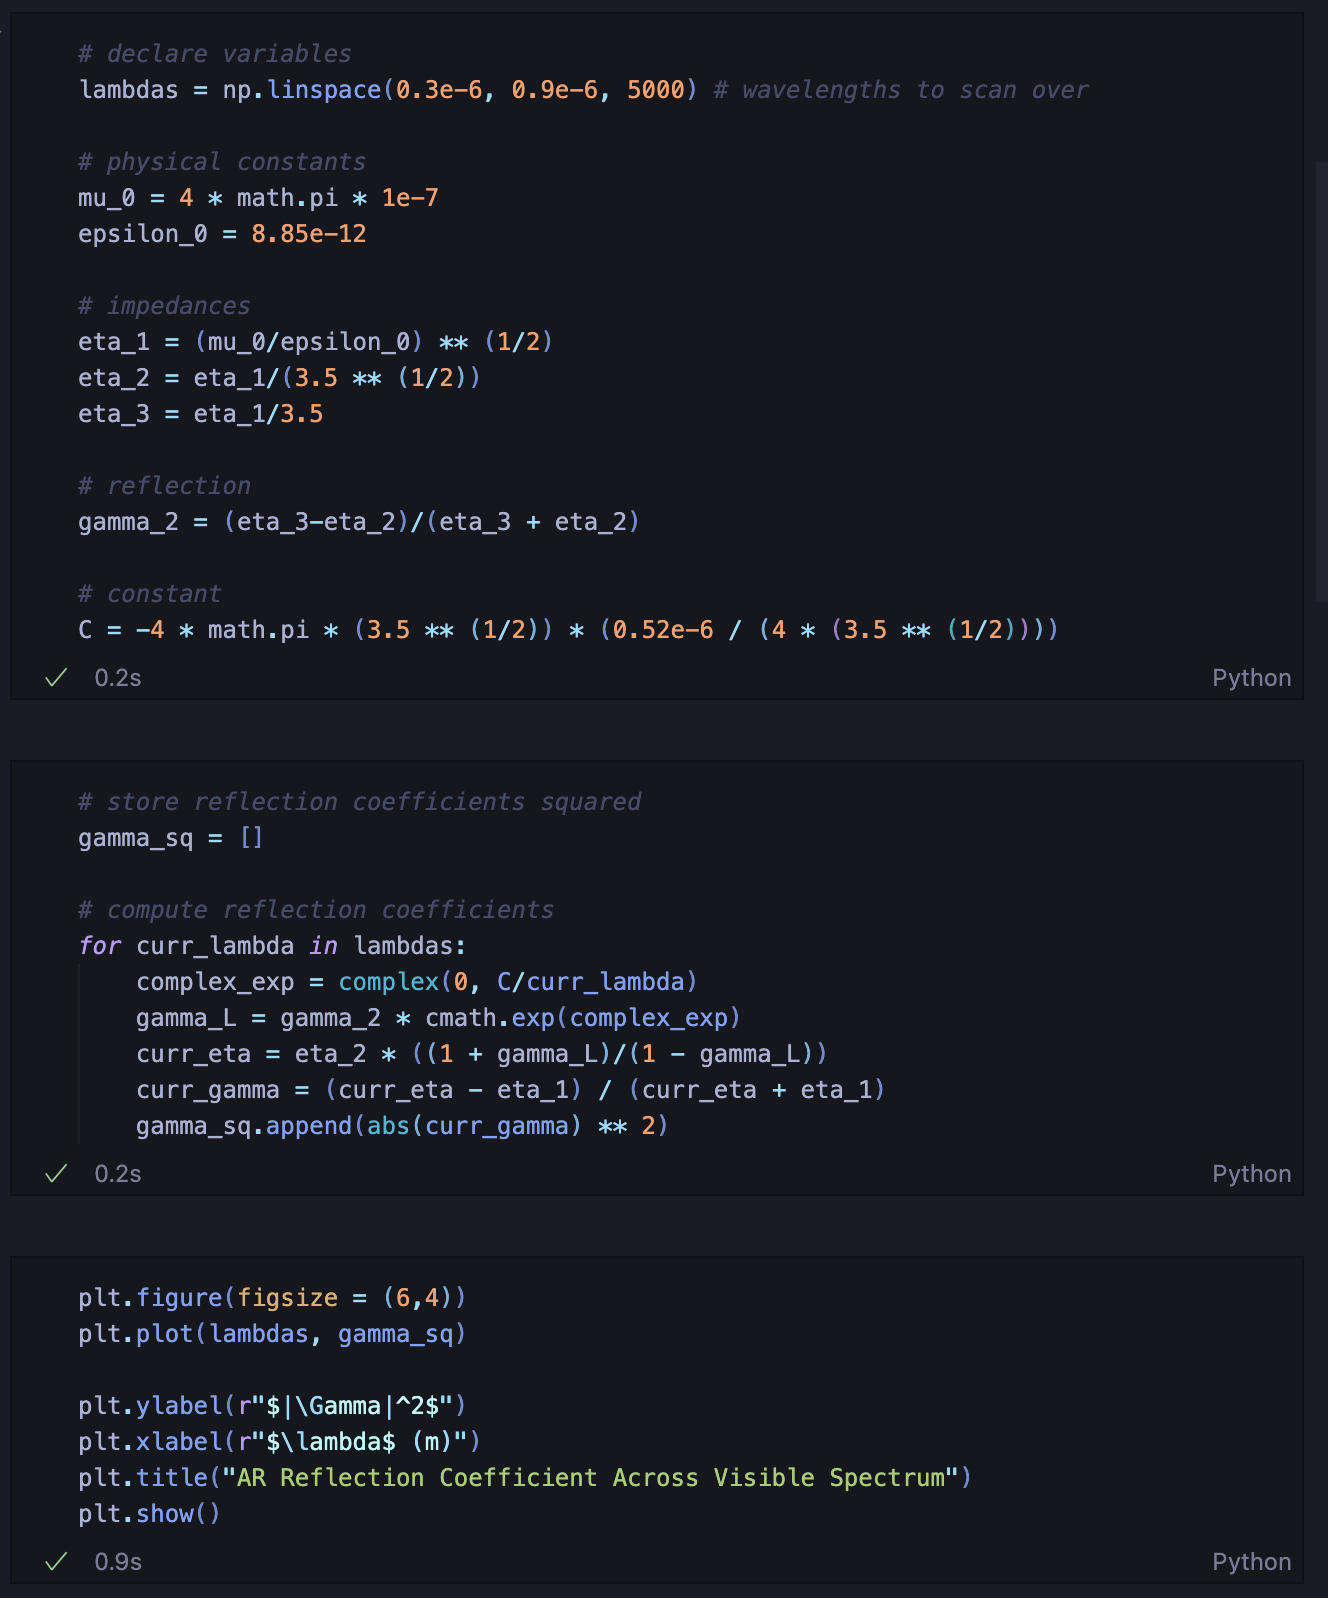
\includegraphics[width = 5in]{images/ece3030-q1-1.png}

		This generates the plot,

		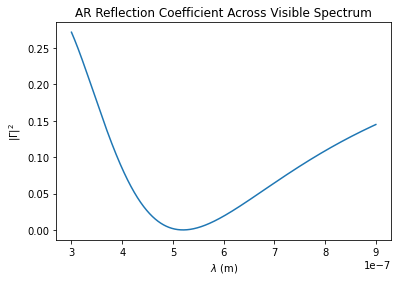
\includegraphics[width = 5in]{images/ece3030-q1-2.png}

	\end{enumerate}

	\item [9.2]
	\begin{enumerate}
		\item [(a)]
		We want the thicknesses of the layers to be $\lambda/4$ where $\lambda$ denotes the wavelength of the design specification light in each layer.
		From question 9.1, we deduced that this $\lambda$ would be given by $\lambda_1/n$ where $\lambda_1$ is the design specification wavelength in vacuum ($0.52 \: \mu \mathrm{m}$) and $n$ is the index of refraction of the material.
		Thus, the length $L_3$ of the $n_3=1.5$ material should be,
		\[L_3 = \frac{\lambda_0}{4n_3}=8.67 \cdot 10^{-8}\:\mathrm{m}\]
		The length $L_2$ of the $n_2=2.4$ material is then,
		\[L_2 = \frac{\lambda_0}{4n_2}=5.42\cdot 10^{-8}\:\mathrm{m}\]
		\[\boxed{\begin{cases}
			L_3 =8.67 \cdot 10^{-8} \: \mathrm{m} \\ 
			L_2 = 5.42 \cdot 10^{-8} \: \mathrm{m}	
		\end{cases}}\]

		\item [(b)]
		We can implement this in Python by finding the transformed impedance after each layer, one at a time.
		Generally, we can do this using the same impedance transformation equation as before.
		We define $\Gamma$ as,
		\[\Gamma = \frac{\eta_L-\eta_0}{\eta_L+\eta_0}\]
		where $\eta_L$ is the impedance "looking in" from the right and $\eta_0$ is the impedance of the layer in question.
		Then by the impedance transformation equation the transformed impedance on the left-side of the layer in question will be,
		\[\eta(z=-L)=\eta_0\frac{1+\Gamma e^{-2j(2\pi/\lambda)L}}{1-\Gamma e^{-2j(2\pi/\lambda)L}}\]
		We know that $\lambda$ in the layer is given by $\lambda_1/n$ where $n$ is the index of refraction of the layer in question.
		Thus, we can rewrite this as,
		\[\eta(z=-L)=\eta_0\frac{1+\Gamma e^{jC/\lambda_1}}{1-\Gamma e^{jC/\lambda_1}}\]
		where,
		\[C=-2\cdot \frac{2\pi\lambda_1}{\lambda}L=-\frac{4\pi\lambda_1}{\lambda_1}nL=-4\pi nL\]
		We iterate through all the layers, and finally find $\Gamma$ by $\Gamma=(\eta_T-\eta_1)/(\eta_T+\eta_1)$ where $\eta_T$ is the "cumulated" transformed impedance.
		We can generate plots for $|\Gamma_1|^2$ over the range of $\lambda_1:[0.3,0.9]\:\mu\mathrm{m}$ with the below Python snippet,

		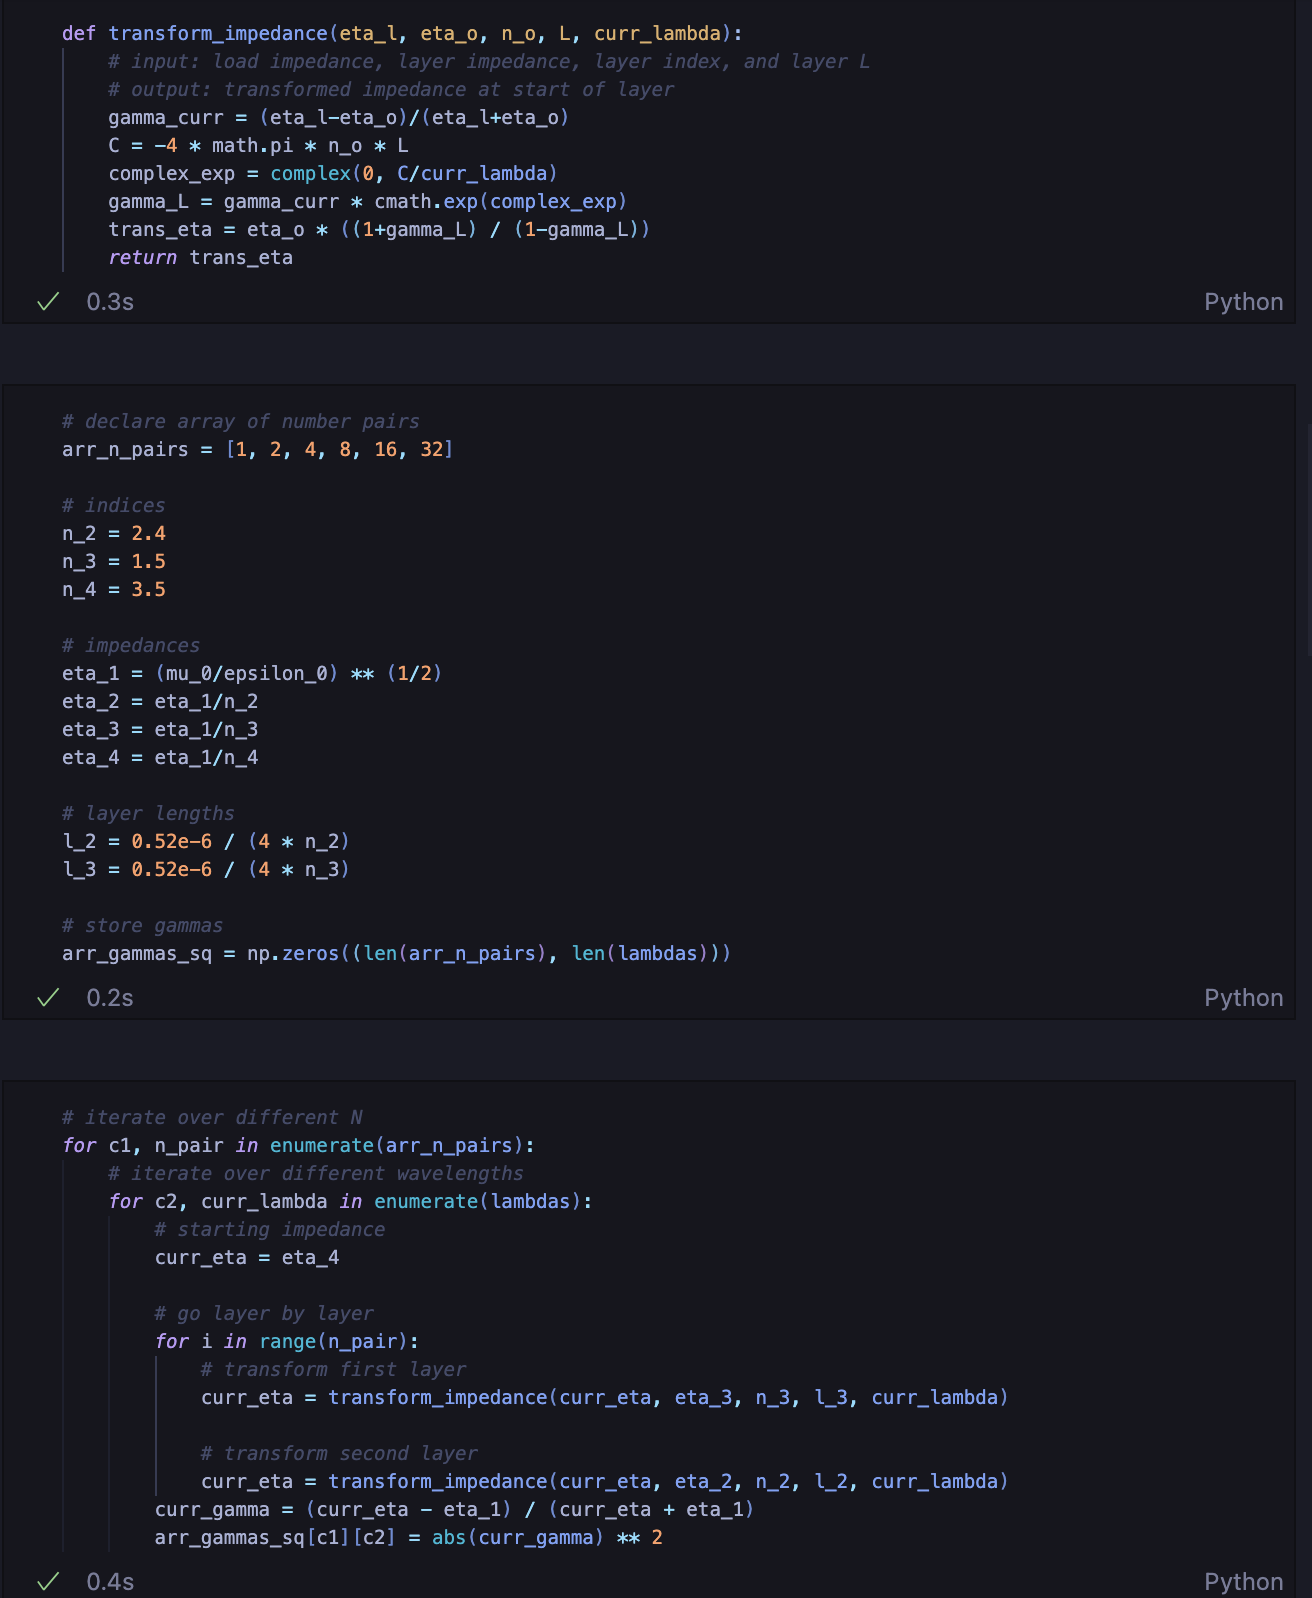
\includegraphics[width = 5in]{images/ece3030-q2-1.png}

		This results in the plots,

		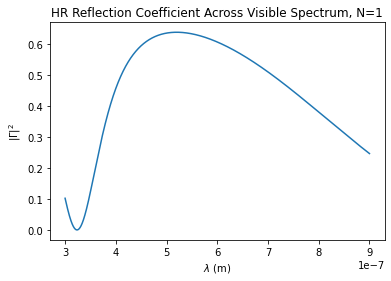
\includegraphics[width = 5in]{images/ece3030-q2-2.png}

		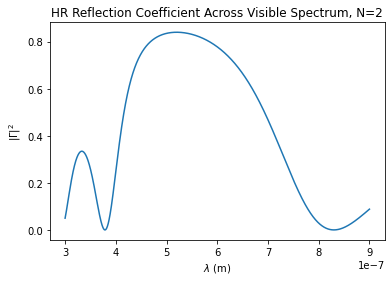
\includegraphics[width = 5in]{images/ece3030-q2-3.png}

		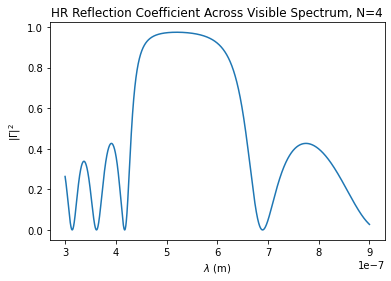
\includegraphics[width = 5in]{images/ece3030-q2-4.png}
		
		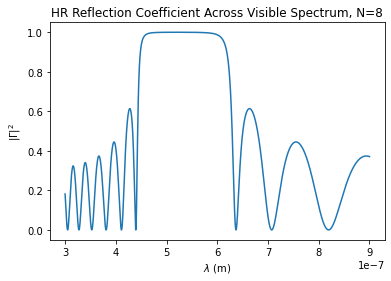
\includegraphics[width = 5in]{images/ece3030-q2-5.png}

		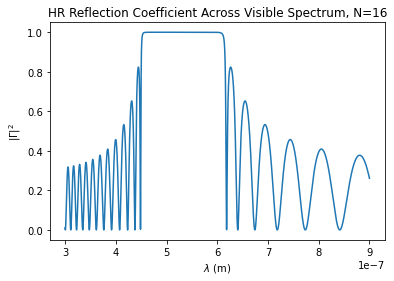
\includegraphics[width = 5in]{images/ece3030-q2-6.png}

		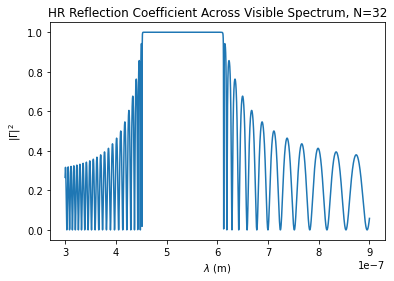
\includegraphics[width = 5in]{images/ece3030-q2-7.png}

		\item [(c)]
		At the design wavelength, we find that the reflection coefficient for our HR design, $\Gamma_{\mathrm{HR}}$, comes out to be,
		\[\Gamma_{\mathrm{HR}} = \frac{\frac{\eta_4}{\eta_1}\left(\frac{\eta_2}{\eta_3}\right)^{2N}-1}{\frac{\eta_4}{\eta_1}\left(\frac{\eta_2}{\eta_3}\right)^{2N}+1}\]
		Computing the numbers, we find that,
		\[|\Gamma_{\mathrm{HR}}|^2=\begin{cases}
			0.639 & N = 1 \\ 
			0.840 & N=2 \\ 
			0.974 & N=4 \\ 
			0.999 & N=8 \\ 
			1.000 & N = 16 \\ 
			1.000 & N=32
		\end{cases}\]
		We can find the reflection coefficient for a conventional mirror, $\Gamma_{\mathrm{MIR}}$, to be,
		\[\Gamma_{\mathrm{MIR}}=\frac{\eta_L-\eta_0}{\eta_L+\eta_0}=\frac{n_0-n_L}{n_0+n_L}\]
		We can perform this simplification because $\mu_0$ is constant.
		From the website, we find that the complex refractive index for aluminum is given by $n_L=0.88783+j6.2810$.
		We also know that the index of refraction in vacuum is given by $n_0=1$.
		Substituting this in via Mathematica, we find that,
		\[|\Gamma_{\mathrm{MIR}}|^2 = 0.917\]
		Thus, we have,
		\[\boxed{|\Gamma_{\mathrm{MIR}}|^2 = 0.917, \; |\Gamma_{\mathrm{HR}}|^2=\begin{cases}
			0.639 & N = 1 \\ 
			0.840 & N=2 \\ 
			0.974 & N=4 \\ 
			0.999 & N=8 \\ 
			1.000 & N = 16 \\ 
			1.000 & N=32
		\end{cases}}\]
		Assuming we use a dielectric HR-coating mirror with at least $N>4$, we should use the dielectric HR-coating mirrors over the metallic (aluminum) mirrors for trapping green light because they have a larger magnitude reflection coefficient $|\Gamma|^2$.
		Because of this, the dielectric HR-coating mirrors are able to keep more of the light "in" the system, and allow the trapped green light to last for the longest amount of time.

	\end{enumerate}

	\item [9.3]
	\begin{enumerate}
		\item [(a)]
		From lecture, we derived that the dispersion relation for $k_z$ for the $\mathrm{TE}_m$ mode is given by,
		\[k_z= \sqrt{\omega^2\mu_0\epsilon-\left(\frac{m\pi}{d}\right)^2}\]
		In order for $k_z$ to not be completely imaginary, and allow the wave to propagate, we seek,
		\[\omega^2\mu_0\epsilon>\left(\frac{m\pi}{d}\right)^2\]
		The cut-off frequency is then given by,
		\[\omega_m=\frac{1}{\sqrt{\mu_0\epsilon}}\left(\frac{m\pi}{d}\right)\]
		Substituting in appropriate values (making sure to use SI units),
		\[\omega_3 = \frac{1}{\sqrt{4\mu_0\epsilon_0}}\frac{3\pi}{0.01}=1.413\cdot 10^{11}\:\mathrm{s^{-1}}\]
		\[\omega_3 = (2\pi)\cdot 1.413\cdot 10^{11}\:\mathrm{Hz}=8.879\cdot 10^{11}\:\mathrm{Hz}\]
		Thus, the cut-off frequency for the $\mathrm{TE}_3$ mode is given by,
		\[\boxed{\omega_{c,3} = (2\pi)\cdot 1.413\cdot 10^{11}\:\mathrm{Hz}=8.879\cdot 10^{11}\:\mathrm{Hz}}\]

		\item [(b)]
		For the $\mathrm{TE}_3$ mode, we set $m=3$, resulting in $k_z$ being,
		\[k_z=\sqrt{\omega^2\mu_0\epsilon-\left(\frac{3\pi}{d}\right)^2}\]
		Substituting this into the formula for $v_p$,
		\[v_p(\omega) = \frac{\omega}{k_z(\omega)}=\frac{\omega}{\sqrt{\omega^2\mu_0\epsilon-(3\pi/d)^2}}=\frac{\omega}{\sqrt{4\omega^2\mu_0\epsilon_0-(3\pi/d)^2}}\]
		If we substitute in numbers from the problem, we find that this is equivalent to,
		\[v_p(\omega) = \frac{\omega}{\sqrt{(4.4485\cdot 10^{-17})\cdot\omega^2-(888264)}}\]
		Thus, we have the phase velocity,
		\[\boxed{v_p(\omega) =\frac{\omega}{\sqrt{4\omega^2\mu_0\epsilon_0-(3\pi/d)^2}} =\frac{\omega}{\sqrt{(4.4485\cdot 10^{-17})\cdot\omega^2-(888264)}}}\]
		Similarly, now computing $v_g$, we can differentiate our expression $k_z$ with respect to $\omega$ to find,
		\[\frac{\partial k(\omega)}{\partial \omega}=\frac{\omega \mu_0\epsilon}{\sqrt{\omega^2\mu_0\epsilon-\left(\frac{3\pi}{d}\right)^2}}\]
		Then,
		\[v_g(\omega)=\left(\frac{\partial k(\omega)}{\partial \omega}\right)^{-1}=\frac{\sqrt{\omega^2\mu_0\epsilon -\left(\frac{3\pi}{d}\right)^2}}{\omega \mu_0\epsilon}=\frac{\sqrt{4\omega^2\mu_0\epsilon_0-\left(\frac{3\pi}{d}\right)^2}}{4\omega \mu_0\epsilon_0}\]
		If we substitute in numbers from the problem, we find that this is equivalent to,
		\[v_g(\omega)=\frac{\sqrt{(4.4485\cdot 10^{-17})\cdot \omega^2-(888264)}}{(4.4485\cdot 10^{-17})\cdot \omega}\]
		Thus, we have the group velocity,
		\[\boxed{v_g(\omega)=\frac{\sqrt{4\omega^2\mu_0\epsilon_0-\left(\frac{3\pi}{d}\right)^2}}{4\omega \mu_0\epsilon_0}=\frac{\sqrt{(4.4485\cdot 10^{-17})\cdot \omega^2-(888264)}}{(4.4485\cdot 10^{-17})\cdot \omega}}\]

		Plotting these via Python, we find that,

		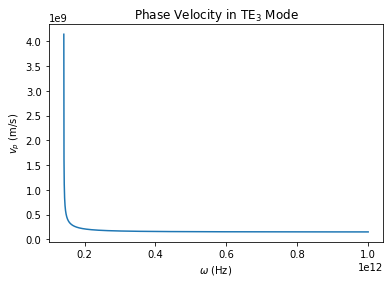
\includegraphics[width = 5in]{images/ece3030-q3-1.png}

		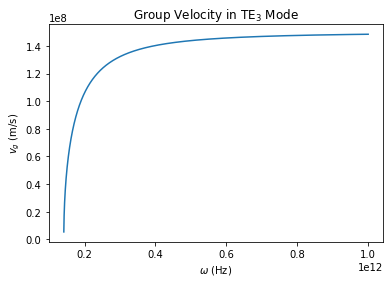
\includegraphics[width = 5in]{images/ece3030-q3-2.png}

		At the cut-off frequency, we notice that the term$\sqrt{4\omega^2\mu_0\epsilon_0-(3\pi/d)^2}=0$.
		Since this term is in the denominator in the phase velocity formula, $v_p\to\infty$ at the cut-off frequency.
		Since this term is in the numerator in the group velocity formula, $v_g\to0$ at the cut-off frequency.
		Thus, at the cut-off frequency, the phase and group velocities are different.
		\[\boxed{\begin{cases}
			\lim_{\omega\to \omega_{c,3}}v_p(\omega)=\infty \\
			\lim_{\omega\to \omega_{c,3}}v_g(\omega)=0 \\
		\end{cases}
		}\]

		If we take the limits of each as $\omega \to \infty$, we find that, by taking the ratio of dominant terms,
		\[\lim_{\omega\to\infty}v_p(\omega)=\lim_{\omega\to\infty}\frac{\omega}{\sqrt{4\omega^2\mu_0\epsilon_0-(3\pi/d)^2}}=\frac{1}{\sqrt{4\mu_0\epsilon_0}}=1.499\cdot 10^8\:\mathrm{m/s}\]
		\[\lim_{\omega\to \infty}v_g(\omega)=\lim_{\omega \to \infty}\frac{\sqrt{4\omega^2\mu_0\epsilon_0-\left(\frac{3\pi}{d}\right)^2}}{4\omega \mu_0\epsilon_0}=\frac{\sqrt{4\mu_0\epsilon}}{4\mu_0\epsilon_0}=\frac{1}{\sqrt{4\mu_0\epsilon_0}}=1.499 \cdot 10^{8}\:\mathrm{m/s}\]
		Thus,
		\[\boxed{\lim_{\omega \to \infty}v_p(\omega)=\lim_{\omega\to\infty}v_g(\omega) = 1.499 \cdot 10^{8}\:\mathrm{m/s}}\]

		\item [(c)]
		For the $\mathrm{TE}_3$ mode, we know that the electric field vector in the waveguide is given by,
		\[\vec E(\vec r)=\hat y E_0\sin\left(\frac{3\pi}{d}x\right)e^{-jk_zz}\]
		Taking the limit of $k_z$ as $\omega \to \omega_{c,3}^+$,
		\[\lim_{\omega \to \omega_{c,3}^+}k_z = \lim_{\omega \to \omega_{c,3}^+}\sqrt{\omega^2\mu_0\epsilon-\left(\frac{3\pi}{d}\right)^2}=0\]
		In other words, this means that our $k$-vector points entirely in the $x$-direction, and does not point in the $z$-direction at all.
		This means that $\lim_{\omega\to\omega_{c,3}^+}\vec k = k_x\hat x=(3\pi/d)\hat x$.
		Substituting this into our equation for the electric field,
		\[\lim_{\omega \to \omega_{c,3}^+}\vec E(\vec r)=\hat y E_0\sin\left(\frac{3\pi}{d}x\right)\]
		Finding the associated magnetic field, we can use the phasor representation where,
		\[\nabla \times \vec E(\vec r)=-j\omega \mu_0\vec H(\vec r)\to \vec H(\vec r)=\frac{\nabla\times \vec E(\vec r)}{-j\omega \mu_0}\]
		Computing $\nabla \times \vec E(\vec r)$ in the limit of the cut-off frequency,
		\[\nabla \times \vec E(\vec r)=\begin{vmatrix}
			\hat x & \hat y & \hat z \\ 
			\partial /\partial x & \partial/\partial y & \partial/\partial z \\ 
			0 & E_0\sin(3\pi x/d) & 0
		\end{vmatrix}=E_0\frac{3\pi}{d}\cos\left(\frac{3\pi}{d}x\right)\hat z\]
		Thus,
		\[\vec H(\vec r)=j\frac{E_0}{\omega\mu_0}\frac{3\pi}{d}\cos\left(\frac{3\pi}{d}x\right)\hat z\]
		We know the time-average power flow density is given by,
		\[\left\langle \vec S(\vec r,t)\right \rangle = \frac{1}{2}\mathrm{Re}\left[\vec E(\vec r)\times (\vec H(\vec r))^*\right]\]
		Taking the complex conjugate of $\vec H(\vec r)$,
		\[(\vec H(\vec r))^*=-j\frac{E_0}{\omega\mu_0}\frac{3\pi}{d}\cos\left(\frac{3\pi}{d}x\right)\hat z\]
		Then, taking the cross product $\vec E(\vec r)\times (\vec H(\vec r))^*$,
		\[\vec E(\vec r)\times (\vec H(\vec r))^*=\begin{vmatrix}
			\hat x & \hat y & \hat z \\ 
			0 & E_0\sin(3\pi x/d) & 0 \\ 
			0 & 0 & -j(E_0/\omega \mu_0)(3\pi/d)\cos(3\pi x/d)	
		\end{vmatrix}\]
		\[\vec E(\vec r)\times (\vec H(\vec r))^*=-j\frac{E_0^2}{\omega \mu_0}\frac{3\pi}{d}\sin\left(\frac{3\pi}{d}x\right)\cos\left(\frac{3\pi}{d}x\right)\]
		We notice that this vector is completely imaginary and has no real part.
		Thus, 
		\[\left\langle \vec S(\vec r, t)\right \rangle = \frac{1}{2}\mathrm{Re}\left[\vec E(\vec r)\times (\vec H(\vec r))^*\right]=0\]
		\[\boxed{\lim_{\omega \to \omega_{c,3}^+}\left\langle \vec S(\vec r,t)\right \rangle = 0}\]
		In other words, the time-average power for the $\mathrm{TE}_3$ mode approaches 0 as the mode approaches its cut-off frequency.
		This makes sense with respect to our phase and group velocity discussion.
		We found that the limit of the group velocity as the frequency approaches the cut-off frequency is $0$.
		The group velocity denotes the velocity at which the "envelope" of the wave travels.
		This corresponds to the velocity at which information or energy in the wave travels.
		Since the group velocity at the cut-off frequency is $0$, this means that no information or energy in the wave should travel, and the wave envelopes act like they are "stuck in place".
		Thus, our result that there is no time-average power for the $\mathrm{TE}_3$ mode when the mode approaches its cut-off frequency makes sense as the group velocity is $0$ which means that wave packets are "frozen" and energy should not travel along the wave.


	\end{enumerate}
			
\end{enumerate}

		

\end{document}
